\chapter{Бизнес-контекст}
\label{ch:chap4}


\section{Профили заинтересованных лиц}
\label{sec:stakeholders}

Заинтересованные лица:
\begin{enumerate}[label=\arabic*]
    \item Владелец предприятия,
    \item Руководитель предприятия,
    \item Руководитель отдела продаж,
    \item Руководитель производственного отдела,
    \item Руководитель отдела логистики,
    \item Логистик,
    \item Клиент.
\end{enumerate}

Профиль ``Владелец предприятия'':

Основная ценность:
\begin{itemize}
    \item Снижение издержек,
    \item Повышение прибыли,
    \item Повышение масштабируемости бизнеса.
\end{itemize}

Профиль ``Руководитель предприятия''

Основная ценность:
\begin{itemize}
    \item Повышение управляемости,
    \item Повышение предсказуемости результатов.
\end{itemize}

Профиль ``Руководителя отдела продаж''

Основные интересы:
\begin{itemize}
    \item Список заказов на дату отдаётся в работу ежедневно не ранее 17:00,
    \item Срочные заказы должны приниматься в работу и после составления плана, но не позднее даты производства на дату доставки, (может привести к пересчету плана),
    \item Отмена заказа должна возможна, но не позднее до даты производства (может привести к пересчету плана),
    \item Возможность указывать временные окна доставки,
    \item Отчет по плановому времени доставки.
\end{itemize}

Профиль ``Руководителя производственного отдела''

Основные интересы:
\begin{itemize}
    \item Логистический план должен быть готов ежедневно к 18:00,
    \item Изменения (пересчет) логистического плана не должен влиять на план производства сформированный на основе исходного логистического плана,
    \item Повышение предсказуемости планирования,
    \item Повышение точности планирования,
    \item Распределение иделий по транспортным контейнерам,
    \item Отчет по порядку погрузки изделий на транспортные контейнеры по-контейнерно.
\end{itemize}

Профиль ``Руководителя отдела логистики'':

Основные интересы:
\begin{itemize}
    \item Ретроспективный анализ исполнения логистических планов,
    \item Хранение планов за текущий и прошлый год.
\end{itemize}

Профиль ``Логистика'':

Основные интересы:
\begin{itemize}
    \item План составляется на конкретную дату,
    \item Автоматическая загрузка заказов на дату доставки,
    \item Ручное добавление заказа по номеру заказа, по клиенту,
    \item Удаление заказа из плана,
    \item Учет заказов не взятых в работу на дату доставки,
    \item Уникальность заказа в плане,
    \item Автоматическая привязка точки доставки заказа к сети дорог общего пользования,
    \item Отчет по плану в целом,
    \item Отчет по маршруту по-машино,
    \item Отчет по порядку погрузки транспортных контейнеров по-машинно,
    \item Отчет по порядку погрузки изделий на транспортные контейнеры по-контейнерно.
\end{itemize}

Профиль ``Клиент'':

Основная ценность:
\begin{itemize}
    \item Получение информации о процессе доставки заказа.
\end{itemize}


\section{Приоритеты проекта}
\label{sec:priorities}

\begin{figure}[H]
    \centering
    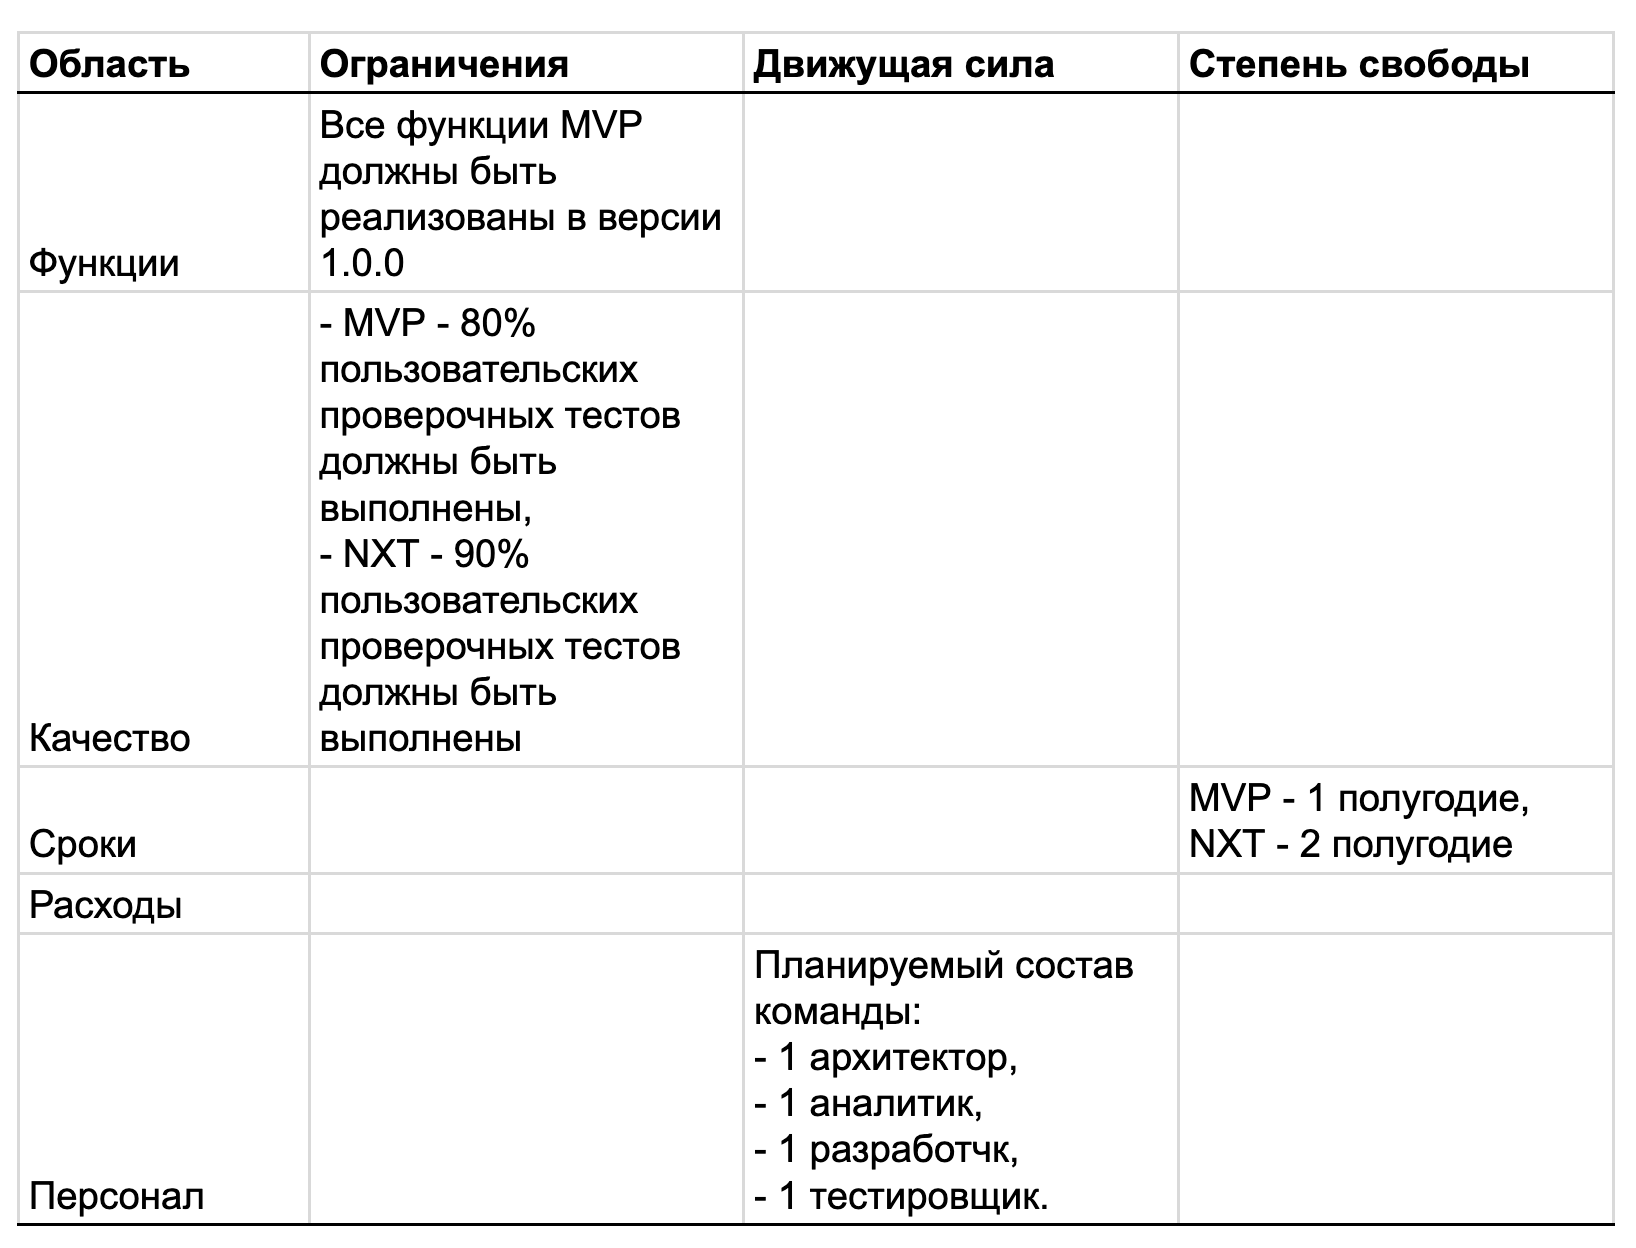
\includegraphics{Снимок экрана 2024-01-17 в 14.59.35}
    \caption{Приоритеты}
    \label{fig:}
\end{figure}


\section{Операционная среда}
\label{sec:env}

Система реализуется согласно микросервисной архитектуре.

Сервера располагаются на оборудовании предприятия.
Сетевой сегмент серверов не должен иметь доступа к сети интернет за исключением исходящих подключений по адресам провайдеров геокодирования.

Внутренние пользователи для коммуникации с системой используют SPA в интернет-браузере.
Рабочие места внутренних пользователей должны иметь доступ к сети интернет как минимум для исходящих подключений по адресам провайдеров картографической информации.

Внешние пользователи для коммуникации с системой используют SPA в интернет-браузере.
Микросервис обслуживания запросов клиентов должен находится в DMZ сегменте сети.

\endinput
